\lstset{language = Java}



\chapter{Einführung}
	\section{Software}
		Software enthält nicht nur ein einziges Programm, sondern unter anderem:
		\begin{itemize}
			\item ein Ausführbares Programm und dessen Daten
			\item Konfigurationsdateien
			\item System Dokumentation (bspw. Architektur, Analyse, Design, \dots)
			\item Nutzerdokumentation (Handbuch)
			\item Support (bspw. Webseite, Telefon, \dots)
			\item \dots
		\end{itemize}
		
		\paragraph{Softwaretypen}
			\begin{description}[leftmargin = 5cm]
				\item[Applikationssoftware] Software, welche direkt mit dem Nutzer interagiert wie Textverarbeitungsprogramme oder komplexe Software wie Steuerverwaltung.
				\item[Systemsoftware] Software, welche üblicherweise nicht direkt mit dem (normalen) Nutzer interagiert, beispielsweise Firmware und Treiber.
				\item[Software as a Service (SaaS)] Serverseitige Software, welche meist über den Browser an den Nutzer ausgeliefert wird.
			\end{description}
		% end
	% end
	
	\section{Bereiche der Softwareentwicklung}
		Zu dem Prozess der Softwareentwicklung gehören:
		\begin{itemize}
			\item \textbf{Software Anforderungen} Erkennung und Definition der Erwartungen an das System und dessen Verhalten.
			\item \textbf{Software Design} Die Struktur der Software (Module, Klassen, API, \dots).
			\item \textbf{Software Qualität} Qualitätssicherung: Einschätzung der Qualität der Software und die Entwicklung, diese zu verbessern.
			\item \textbf{Testen, Verifikation und Validierung der Software} Die systematische Erkennung (und Eliminierung) von Fehlern.
			\item \textbf{Software Wartung} Der Betrieb der Software, die Weiterentwicklung und die Anpassung an neue Anforderungen und Umgebungen.
			\item \textbf{Software Konfiguration und Management} Verwaltung von unterschiedlichen Versionen und Konfigurationen der Software.
			\item \textbf{Softwareentwicklungstools und -methoden} UML Tools, IDEs, Versionskontrollsysteme, Aufgabenverwaltung, Statische Analyse, \dots
			\item \textbf{Softwareentwicklungsprozesse} Definition und Verbesserung des Enwticklungsprozesses.
		\end{itemize}
	% end
% end

\chapter{Softwareprozesse}
	\section{Grundlegende Begriffe}
		\subsection{Grundlegende Schritte in der Softwareentwicklung}
			\begin{description}
				\item[Anforderungsspezifikation] Definition der Software, welche entwickelt werden soll und die Einschränkungen dieser Operation.
				\item[Entwicklung] Design und Implementierung der Software.
				\item[Validierung] Sicherung, dass die Software erfüllt, was der Kunde verlangt.
				\item[Evolution] Adaption und Modifikation der Software, um mit Änderungen des Kunden oder der Marktbedingungen umzugehen.
			\end{description}
		% end
	% end

	\section{Projektplanung}
		\subsection{Diagramm: Aktivitätsdiagramm}
			\label{diagram:activity}

			\paragraph{Beschreibung}
				Ein Aktivitätendiagramm stellt die Abhängigkeiten zwischen Aktivitäten und Meilensteinen als Graph dar, aus welchem Schlüsse über die Projektdauer gezogen werden können.
			% end
			
			\paragraph{Beispiel}
				In Abbildung \ref{fig:activity} ist ein Beispiel für ein Aktivitätendiagramm mit den Aktivitäten T1, T2, T3, T4, T5 und T6 und den Meilensteinen M1 und M2 gegeben.
				
				In Abbildung \ref{fig:activitycritical} wurden die kritischen Pfade markiert.

				\begin{figure}[ht]
					\centering
					\begin{tikzpicture}[
								->,
								line width = 0.5mm,
								every node/.style = {
									draw,
									minimum height = 40pt,
									minimum width = 60pt,
									align = center
								},
								start/.style = {
									rounded corners = 0.2cm,
									fill = TUDa-8a
								},
								release/.style = {
									rounded corners = 0.2cm,
									fill = TUDa-4a
								},
								milestone/.style = {
									rounded corners = 0.2cm,
									fill = TUDa-0\IfDarkModeTF{c}{b}
								}
							]
						\node [start] (start) {Start};
						\node [right = of start] (T2) {T2 \\ 10 Tage};
						\node [above = of T2] (T1) {T1 \\ 8 Tage};
						\node [below = of T2] (T3) {T3 \\ 15 Tage};
						\node [right = of T2] (T4) {T4 \\ 6 Tage};
						\node [milestone, above = of T4] (M1) {M1};
						\node [milestone, below = of T4] (M2) {M2};
						\node [right = of T4] (T5) {T5 \\ 3 Tage};
						\node [below = of T5] (T6) {T6 \\ 5 Tage};
						\node [release, right = of T5] (release) {Release};
						
						\draw (start) -- (T1);
						\draw (start) -- (T2);
						\draw (start) -- (T3);
						\draw (T1) -- (M1);
						\draw (T2) -- (M1);
						\draw (T3) -- (M2);
						\draw (M1) -- (T4);
						\draw (T4) -- (M2);
						\draw (M2) -- (T5);
						\draw (M2) -- (T6);
						\draw (T5) -- (release);
						\draw (T6) -- (release);
					\end{tikzpicture}
					\caption{Aktivitätsdiagramm: Beispiel}
					\label{fig:activity}
				\end{figure}

				\begin{figure}[ht]
					\centering
					\begin{tikzpicture}[
								->,
								line width = 0.5mm,
								every node/.style = {
									draw,
									minimum height = 40pt,
									minimum width = 60pt,
									align = center
								},
								start/.style = {
									rounded corners = 0.2cm,
									fill = TUDa-8a
								},
								release/.style = {
									rounded corners = 0.2cm,
									fill = TUDa-4a
								},
								milestone/.style = {
									rounded corners = 0.2cm,
									fill = TUDa-0\IfDarkModeTF{c}{b}
								}
							]
						\node [start] (start) {Start};
						\node [right = of start] (T2) {T2, 10 Tage};
						\node [above = of T2] (T1) {T1, 8 Tage};
						\node [below = of T2] (T3) {T3, 15 Tage};
						\node [right = of T2] (T4) {T4, 6 Tage};
						\node [milestone, above = of T4] (M1) {M1};
						\node [milestone, below = of T4] (M2) {M2};
						\node [right = of T4] (T5) {T5, 3 tage};
						\node [below = of T5] (T6) {T6, 5 Tage};
						\node [release, right = of T5] (release) {Release};

						\draw (start) -- (T1);
						\draw [TUDa-9\IfDarkModeTF{a}{c}] (start) -- (T2);
						\draw (start) -- (T3);
						\draw (T1) -- (M1);
						\draw [TUDa-9\IfDarkModeTF{a}{c}] (T2) -- (M1);
						\draw (T3) -- (M2);
						\draw [TUDa-9\IfDarkModeTF{a}{c}] (M1) -- (T4);
						\draw [TUDa-9\IfDarkModeTF{a}{c}] (T4) -- (M2);
						\draw (M2) -- (T5);
						\draw [TUDa-9\IfDarkModeTF{a}{c}] (M2) -- (T6);
						\draw (T5) -- (release);
						\draw [TUDa-9\IfDarkModeTF{a}{c}] (T6) -- (release);
					\end{tikzpicture}
					\caption{Aktivitätsdiagramm: Beispiel mit markiertem kritischen Pfad (rot)}
					\label{fig:activitycritical}
				\end{figure}
			% end
			
			\paragraph{Metriken}
				\begin{description}
					\item[Kritischer Pfad] Der längste Pfad zwischen Start- und Endpunkt. Sollten sich Aktivitäten auf dem kritischen Pfad verspäten, verspätet sich das gesamte Projekt. In Abbildung \ref{fig:activitycritical} wurde der kritische Pfad zwischen Start und Release markiert.
				\end{description}
			% end
		% end
		
		\subsection{Diagramm: Gantt Chart}
			\label{diagram:gantt}
			
			\paragraph{Beschreibung}
				Ein Gantt Char stellt die Aktivitäten in einem Projekt im zeitlichen Verlauf in Relation zu den Meilensteinen dar.
				
				Das Beispiel in \ref{fig:gantt} stellt das Aktivitätendiagramm aus \ref{fig:activity} als Gantt Chart dar.
			% end
			
			\paragraph{Beispiel}
				\begin{figure}[ht]
					\centering
					\begin{ganttchart}[
						title/.append style={fill=\thepagecolor},
						bar/.append style={fill=\thepagecolor},
						canvas/.append style={fill=\thepagecolor},
						vgrid,
						]{1}{21}
						\gantttitle{M1}{10}
						\gantttitle{M2}{6}
						\gantttitle{Release}{5}
						\\
						\ganttbar{T1}{1}{8} \\
						\ganttbar{T2}{1}{10} \\
						\ganttbar{T3}{1}{15} \\
						\ganttbar{T4}{11}{16} \\
						\ganttbar{T5}{17}{19} \\
						\ganttbar{T6}{17}{21}
					\end{ganttchart}
					\caption{Gantt Chart: Beispiel}
					\label{fig:gantt}
				\end{figure}
			% end
		% end
	% end

	\section{Projektmanagement}
		\subsection{Prozessmodelle}
			Softwareprozessmodelle sind simplifizierte und abstrakte Beschreibungen eines Entwicklungsprozesses, welche eine Sicht auf die Entwicklung darstellen. Sie enthalten Aktivitäten innerhalb der Entwiclung, Softwareprodukte (bspw. Architekturbeschreibungen), Quellcode, Nutzer-Dokumentation und die Rollen der an der Entwicklung beteiligten Personen.
			
			Beispiele für Prozessmodelle sind:
			\begin{itemize}
				\item Waterfall
				\item Spiral
				\item V-Model (XT)
				\item eXtreme Programming
			\end{itemize}
		% end
		
		\subsection{Aktivitäten}
			\begin{itemize}
				\item Projektplanung
				\item Kostenabschätzung
				\item Projektüberwachung und -sichtigungen
				\item Personalselektion und -evaluierung
				\item Präsentation
			\end{itemize}
		% end
		
		\subsection{Projektplanung}
			Ein Softwareprojekt enthält viele Pläne, wobei ein guter Startplan mit allen vorliegenden Informationen Vorraussetzung ist für das Gelingen des Projektes.
			
			Es gibt viele Unterschiedliche Pläne, bspw.:
			\begin{itemize}
				\item \textbf{Projektplan} Siehe Sektionen \enquote{Projektplan} (\ref{ssec:projektplan}).
				\item \textbf{Qualitätssicherungsplan} Beschreibung, welche Qualitätssicherungsprozeduren und Standards genutzt werden.
				\item \textbf{Personalentwicklungsplan} Beschreibt, wie die Fähigkeiten und Erfahrungen der einzelnen Mitarbeiter und des Teams eingesetzt und weiterentwickelt werden.
			\end{itemize}
			
			\subsubsection{Projektplan}
				\label{ssec:projektplan}
				
				\paragraph{Struktur}
					\begin{description}[leftmargin = 5cm]
						\item[Einleitung] Ziele des Projektes und Einschränkungen (Zeit, Budget, \dots).
						\item[Projektorganisation] Organisation des Entwicklungsteams, die eingebundenen Personen und deren Rollen.
						\item[Risikoanalyse] Mögliche Projektrisiken, deren Eintrittswahrscheinlichkeit und Risikominderungsstrategien.
						\item[Resourcenanforderungen] Nötige Hard- und Software für das Durchführen des Projektes.
						\item[Arbeitsaufteilung] Aufteilung des Projektes in Aktivitäten, Identifikation von Meilensteinen und Ergebnisse jeder Aktivität.
						\item[Zeitplan] Abhängigkeiten zwischen Aktivitäten, geschätzte Zeit bis zu jedem Meilenstein und die Zuweisung von Personen zu Aktivitäten.
						\item[Mechanismen zur Überwachung und Mitteilung]
					\end{description}
				% end
				
				Die Aktivitäten können in einem Aktivitätendiagramm (\enquote{Activity Diagram}) dargestellt werden, siehe \ref{diagram:activity}.
			% end
		% end
	
		\subsection{Prozessmodell: Wasserfall}
			\subsubsection{Beschreibung}
				Die folgenden Aktivitäten werden strikt in der folgenden Reihenfolge abgearbeitet und der nächste Schritt wartet auf den vorherigen:
				\begin{enumerate}
					\item Anforderungsdefinition
					\item System- und Softwaredesign
					\item Implementation und Unittests
					\item Integrations- und Systemtests
					\item Inbetriebnahme und Wartung
				\end{enumerate}
			
				Sollten Fehler in einer Phase auftreten, so wird diese gestoppt und die vorherige Phase muss wiederholt werden. Sommit fließen die Ergebnisse aller Phasen in die vorherigen ein, wie in \ref{fig:waterfall} zu sehen ist.
			
				\begin{figure}[ht]
					\centering
					\begin{tikzpicture}
						\node [] (stage1) {Anforderungsdefinition};
						\node [below = of stage1] (stage2) {System- und Softwaredesign};
						\node [below = of stage2] (stage3) {Implementation und Unittests};
						\node [below = of stage3] (stage4) {Integrations- und Systemtests};
						\node [below = of stage4] (stage5) {Inbetiebnahme und Wartung};
						
						\coordinate [left = of stage3] (dotleft);
						
						\draw [->] (stage1) -- (stage2);
						\draw [->] (stage2) -- (stage3);
						\draw [->] (stage3) -- (stage4);
						\draw [->] (stage4) -- (stage5);
						\draw [->] (dotleft) |- (stage4);
						\draw [->] (dotleft) |- (stage3);
						\draw [->] (dotleft) |- (stage2);
						\draw [->] (dotleft) |- (stage1);
						\draw (stage5) -| (dotleft);
					\end{tikzpicture}
					\caption{Prozessmodell: Waterfall}
					\label{fig:waterfall}
				\end{figure}
			% end
			
			\subsection{Kritik}
				\begin{itemize}
					\item Kein iterativer Prozess
					\item Änderung von Anforderungen und Design schwierig und Zeitaufwändig
					\item Das Testen der Software startet erst in späteren Phasen $ \implies $ Fehler werden erst spät erkannt
					\item Einzelne Phasen werden von unterschiedlichen Teams vorangetrieben, welche später möglicherweise nicht mehr zur Verfügung stehen können.
				\end{itemize}
			% end
		% end
		
		\subsection{V-Modell}
			Siehe \ref{fig:vmodel}.
			
			Nachteil: Bei einem V-Modell wird 50\% des Budgets für das V-Modell ausgegeben.

			\begin{figure}[ht]
				\centering
				\begin{tikzpicture}[->, every node/.style = { draw, text width = 3cm, minimum height = 2cm, align = center }]
					\node [x = 0, y = 0] (l5) {Implementation};
					\node [above left = of l5] (l41) {Detailliertes Design};
					\node [left of = l41, above = 2cm] (l31) {System Design};
					\node [left of = l31, above = 2cm] (l21) {System Spezifikation};
					\node [left of = l21, above = 2cm] (l11) {Anforderungs Spezifikation};
					
					\node [above = of l5] (l42) {Modul/Unit Testplan};
					\node [above = of l42] (l32) {Untersystem Integrations Testplan};
					\node [above = of l32] (l22) {System Integrations Plan};
					\node [above = of l22] (l12) {Akzeptanz Testplan};
					
					\node [above right = of l5] (l43) {Modul/Unit Tests};
					\node [right of = l43, above = 2cm] (l33) {Untersystem Integrations Test};
					\node [right of = l33, above = 2cm] (l23) {System Integrations Test};
					\node [right of = l23, above = 2cm] (l13) {Akzeptanz Tests};
					
					\draw (l11) -- (l12);
					\draw (l11) -- (l21);
					\draw (l21) -- (l12);
					\draw (l21) -- (l22);
					\draw (l21) -- (l31);
					\draw (l31) -- (l22);
					\draw (l31) -- (l32);
					\draw (l31) -- (l41);
					\draw (l41) -- (l32);
					\draw (l41) -- (l42);
					\draw (l41) -- (l5);
					\draw (l5) -- (l42);
					\draw (l5) -- (l43);
					\draw (l43) -- (l33);
					\draw (l33) -- (l23);
					\draw (l23) -- (l13);
					\draw (l12) -- (l13);
					\draw (l22) -- (l23);
					\draw (l32) -- (l33);
					\draw (l42) -- (l43);
				\end{tikzpicture}
				\caption{V-Modell}
				\label{fig:vmodel}
			\end{figure}
		% end
		
		\subsection{Agile Entwicklung}
			\info{\textbf{Ziel:} Möglichst schnelle Entwicklung von Software und Einarbeitung von Änderungen der Anforderungen}
		
			\begin{itemize}
				\item Höchste Priorität hat das Zufriedenstellen des Kunden
				\item Regelmäßige Auslieferung von Zwischenständen (bspw. alle zwei Wochen)
				\item Funktionierende Software ist das Primärziel und der Fortschritt (30\% Implementiert $ \rightarrow $ 30\% des Projektes abgeschlossen)
				\item Einfachheit ist essentiell
				\item Änderungen der Anforderungen
				\item Das Team reflektiert in regelmäßigen Abständen, um effektiver zu werden
				\item Manager und Entwickler müssen zusammen arbeiten
			\end{itemize}
		% end
		
		\subsection{Prozessmodell: eXtreme Programming (XP)}
			In XP wird in kurzen Iterationen gearbeitet, wobei in jeder Iteration bestimmte User Stories abgearbeitet werden. Die abzuarbeitenden User Stories werden in der Iterationsplanung festgelegt.

			\subsubsection{User Stories}
				Der essentielle Teil der Entwicklung. Eine User Story beschreibt eine Anforderung. Eine User Story wird anschließend in einzelne Tasks aufgebrochen.
				
				\begin{itemize}
					\item User Stories müssen für den Kunden verständlich sein
					\item Jede User Story muss von Wert sein für den Kunden
					\item User Storie sollten so umfangreich sein, dass man einige abarbeiten kann pro Iteration
					\item User Stories sollten unabhängig sein
					\item Jede User Story muss testbar sein
					\item Jeder User Story werden \textit{Story Points} zugewiesen, welche ein abstraktes Zeitmaß darstellen zur Einschätzung der Bearbeitungsdauer
					\item In jeder User Story sollte ein Akzeptanzkriterium gegeben sein
				\end{itemize}
				
				\noindent Langes Template: Als ein <Rolle> möchte ich <Ziel> sodass <Vorteile>. \\
				Kurzes Template: Als ein <Rolle> möchte ich <Ziel>.
			% end
			
			\subsubsection{Entwicklung}
				\paragraph{Testgetriebene Entwicklung}
					Jede Implementierung startet mit der Entwicklung von Tests, sodass die Implementierung korrekt ist, sobald alle Tests funktionieren.
				% end
				
				\paragraph{Kontinuierliche Integration}
					Entwickler checken ihren Code regelmäßig ein (mehrmals am Tag), sodass ein CI-Server regelmäßig Tests ausführen kann (automatisierte Tests und Build System).
				% end
				
				\paragraph{Pair Programming}
					Code ist von genau zwei Entwicklern geschrieben
					\begin{itemize}
						\item Einer fokussiert sich auf den besten Weg der Implementierung
						\item Der andere fokussiert sich auf den Code (aus einer strategischen Sicht)
					\end{itemize}
				% end
			% end
			
			\subsubsection{Planung}
				\paragraph{Initiale Planung (Start des Projektes)}
					\begin{itemize}
						\item Entwickler und Kunden arbeiten gemeinsam die relevanten User Stories heraus
						\item Entwickler schätzen die Story Points für jede User Story \\
							  {\small Eine User Story mit doppelt so vielen Story Points wie eine andere sollten doppelt so lange dauern.}
						\item Für eine genaue Zeitabschätzung ist die \textit{Velocity} (Story Points pro Zeit) erforderlich, diese wird mit der Zeit genauer (eine Prototyp-Implementierung zur Messung der Velocity nennt sich \textit{Spike})
					\end{itemize}
				% end
				
				\paragraph{Release Planung}
					\begin{itemize}
						\item Entwickler und Kunden einigen sich auf ein Datum für das erste Release (2-4 Monate)
						\item Kunden entscheiden sich für grobe Zusammensetzung der User Stories (unter Beachtung der Velotiy)
						\item Wird die Velocity genauer, wird der Releaseplan geändert
					\end{itemize}
				% end
				
				\paragraph{Iterations Planung}
					\begin{itemize}
						\item Der Kunde sucht die User Stories für die Iteration
						\item Die Reihenfolge der Abarbeitung ist eine technische Entscheidung
						\item Die Iteration endet an einem bestimmten Tag, auch wenn nicht alle Stories abgearbeitet wurden
						\item Die Schätzung für alle \textit{erfolgreich abgearbeiteten} Stories wird summiert und die Velocity berechnet
						\item Die geplante Velocity der nächsten Iteration basiert auf der Velocity der vorherigen Iteration
					\end{itemize}
					
					\begin{equation*}
						\text{Velocity} = \frac{\text{Summe an Story Points}}{\text{Summe der verbrauchten Zeit pro User Story in einer Iteration}}
					\end{equation*}
				% end
				
				\paragraph{Aufgaben Planung}
					\begin{itemize}
						\item Stories werden auf Aufgaben (Tasks) heruntergebrochen, welche 4h bis 16h benötigen
						\item Jeder Entwickler kann sich Aufgaben aussuchen
					\end{itemize}
				% end
			% end
		% end
	% end
	
	\section{Anforderungsanalyse}
		\label{sec:anforderungsanalyse}
	
		Anforderungen sind Beschreibungen der Dienste, welche von dem System zur Verfügung gestellt werden sollen und die Einschränkungen des selbigen. Die Anforderungsanalyse beschäftigt sich mit
		\begin{itemize}
			\item dem Erkennen,
			\item der Analyse,
			\item der Dokumentation und
			\item der Validierung
		\end{itemize}
		der Anforderungen. Der Prozess ist in \ref{fig:reqeng} aufgezeigt.
		
		Diese Anforderungen werden in einem sogenannten Pflichtenheft (eng. \enquote{System Requirements Specification}) niedergeschrieben.
		
		\begin{figure}[ht]
			\centering
			\begin{tikzpicture}[
						->,
						every node/.style = {
							draw,
							align = center,
							text width = 3.5cm,
							minimum height = 1.5cm
						},
						activity/.style = {
							fill = TUDa-6\IfDarkModeTF{c}{a},
						}
					]
				\node [activity] (feasibility) {Machbarkeitsstudie};
				\node [activity, right = of feasibility] (analysis) {Anforderungsanalyse};
				\node [activity, right = of analysis] (spec) {Anforderungs- spezifikation};
				\node [activity, right = of spec] (valid) {Anforderungs- validierung};
				\node [below = 3 of feasibility] (feasibilityReport) {Machbarkeitsbericht};
				\node [below = 1 of analysis] (systemModels) {Systemmodelle};
				\node [below = 3 of spec] (requirements) {Nutzer- und Systemanforderungen};
				\node [below = 5 of valid] (requirementsDoc) {Anforderungs- dokument};
				
				\draw (feasibility) -- (analysis);
				\draw (analysis) -- (spec);
				\draw (spec) -- (analysis);
				\draw (spec) -- (valid);
				\draw (valid) -- (spec);
				\draw (feasibility) -- (feasibilityReport);
				\draw (analysis) -- (systemModels);
				\draw (spec) -- (requirements);
				\draw (valid) -- (requirementsDoc);
				\draw (systemModels) |- (requirementsDoc);
				\draw (requirements) |- (requirementsDoc);
			\end{tikzpicture}
			\caption{Anforderungsanalyse: Arbeitsablauf}
			\label{fig:reqeng}
		\end{figure}

		\subsection{Anforderungstypen}
			\subsubsection{Nutzeranforderungen}
				\begin{itemize}
					\item Natürlicher Sprache oder Diagramme
					\item Oftmals auf einem hohen Level und abstrakt (meist von dem Kunden geschrieben)
					\item Beschreibung von:
						\begin{itemize}
							\item Diensten
							\item Produktionseinschränkungen
						\end{itemize}
				\end{itemize}
				
				\paragraph{Beispiel}
					Das Büchereisystem soll alle Daten halten, welche zur Lizensierung nötig sind.
				% end
			% end
			
			\subsubsection{Systemanforderungen}
				\begin{itemize}
					\item Präzise und detaillierte Beschreibungen
					\item Meist von dem Entwickler geschrieben
					\item Beschreibung von:
						\begin{itemize}
							\item Funktionen und Diensten
							\item Einschränkungen
						\end{itemize}
				\end{itemize}
				
				\paragraph{Beispiele}
					Alle Anfragen an das System sollen fünf Jahre gespeichert werden.
				% end
			% end
			
			\subsubsection{Domänenanforderungen}
				Domänenanforderungen sind meist nicht von dem Kunden oder dem Entwickler spezifiziert, sondern von der jeweiligen Anforderungsdomäne.
				
				\begin{itemize}
					\item Meist ausgedrückt in Domänen-spezifischen Sprachen und daher für den Softwareentwickler schwer zu verstehen.
					\item Von Domänen-Experten oftmals implizit angenommen.
				\end{itemize}
				
				\paragraph{Beispiel}
					Neue Veröffentlichungen in der Bücherei sollen automatisch an die nationale Bibliothek geleitet werden.
				% end
			% end
		% end
		
		\subsection{Anforderungsklassifizierungen}
			Die Anforderungen (Nutzeranforderungen, Systemanforderungen, Domänenanforderungen) können jeweils noch in \textit{funktionale} und \textit{nichtfunktionale} Anforderungen klassifiziert werden.
			
			\subsubsection{Funktionale Anforderungen}
				Funktionale Anforderungen spezifizieren
				\begin{itemize}
					\item die Dienste, welche das System zur Verfügung stellt,
					\item die Reaktion des Systems auf bestimmte Eingaben und
					\item das Verhalten des Systems in bestimmten Situationen.
				\end{itemize}
				
				\paragraph{Beispiel}
					Wenn der Nutzer den Knopf \enquote{Seite Anlegen} drückt, wird eine neue Seite angelegt.
				% end
			% end
			
			\subsubsection{Nichtfunktionale Anforderungen}
				Nichtfunktionale Anforderungen spezifizieren Einschränkungen der Dienste/Funktionen des Systems, welche oftmals nicht vollständig von Tests abgedeckt werden können:
				\begin{itemize}
					\item Produktanforderungen
						\begin{itemize}
							\item Portabilität
							\item Verlässlichkeit
							\item Effizienz (Performanz, Speicherplatz, \dots)
							\item Nutzbarkeit
						\end{itemize}
					\item Organisatorische Anforderungen
						\begin{itemize}
							\item Auslieferung
							\item Implementation
							\item Nutzung von Standards (ISO, IEEE, \dots)
						\end{itemize}
					\item Externe Anforderungen
						\begin{itemize}
							\item Interoperabilität
							\item Ethik
							\item Recht (Sicherheit, Datenschutz, \dots)
						\end{itemize}
				\end{itemize}
				
				Nichtfunktionale Anforderungen sind oftmals großflächige Anforderungen, welche das gesamte System betreffen. Allerdings sind solche Anforderungen meistens kritischer als funktionale Anforderungen (bspw. \enquote{Das System soll sicher vor Angriffen sein.}).
				
				Um nichtfunktionale Anforderungen überprüfbar zu machen, ist oftmals eine Umformulierung oder Abänderung der eigentlichen Anforderung nötig. Hierdurch können auch funktionale Anforderungen aufgedeckt werden.
				
				\paragraph{Beispiel}
					Die Oberfläche soll ansprechend und einfach zu bedienen sein.
				% end
			% end
		% end
	% end
	
	\section{Anwendungsfälle}
		Anwendungsfälle beschreiben, wie ein Angehöriger einer Rolle (\textit{Akteur}) das System in einem bestimmten \textit{Szenario} nutzt.
		
		\subsection{\enquote{Fully Dressed} Use Case}
			Ein \textit{Fully Dressed Use Case} beschreibt einen Anwendungsfall sehr genau und sieht folgendermaßen aus:
			
			\begin{table}[ht]
				\begin{tabular}{l l}
					Abschnitt & Beschreibung / Einschränkungen \\
					\hline
					Use Case Name & Der Name des Anwendungsfalls / Startet mit einem Verb \\
					Bereich & Betroffene Bereiche des Systems \\
					Ebene & Abstraktionsebene / Nutzerziel, Zusammenfassung oder Unterfunktion \\
					Primärakteur & Initiator des Anwendungsfalls \\
					Stakeholder & Personen, die dieser Anwendungsfall betrifft \\
					Vorbedingungen & \\
					Akzeptanzkriterien & Korrektheit der Implementierung \\
					Erfolgskriterien & Nice-to-Have \\
					Hauptszenario & Typische Schritte, des Anwendungsfalls / Nummerierte Liste \\
					Erweiterungen & Alternative Erfolgs- und Fehlschlagszenarien / Fehlschlagspunkte des Hauptszenarios \\
					Spezialanforderungen & Verwandte, nichtfunktionale Anforderungen \\
					Technologien & Einzusetzende Technologien \\
					Häufigkeit & Häufigkeit des Eintretens des Anwendungsfalls \\
					Anderes & Bspw. offene Tickets \\
				\end{tabular}
				
				\begin{itemize}
					\item Ebene
						\begin{description}
							\item[Nutzerziel] Wichtigste Ziele; Essentielle Ziele des Nutzers
							\item[Zusammenfassung] Beschreibt den Kontext mehrerer Nutzerziele
							\item[Unterfunktion] Anwendungsfälle, welche Teil eines anderen Nutzerziels sind
						\end{description}
				\end{itemize}
			\end{table}
		% end
		
		\subsection{Diagramm: Use Case (UML)}
			\label{diagram:umlusecase}
			
			{ \footnotesize UML Specification Version 2.5.1, Chapter 18}
			
			\paragraph{Beschreibung}
				Ein Use Case Diagramm stellt Anforderungsfälle und deren Relation zu dem System und den Akteuren dar.
				
				Im Diagramm \ref{fig:usecase} ist ein Beispiel für ein Use Case Diagramm gegeben. Im folgenden werden die einzelnen Teile erläutert.
				
				\begin{tikzpicture}[item/.style = { minimum width = 4cm }, desc/.style = { text width = 8cm, align = left }]
					\umlactor[item]{Akteur}
					\umlusecase[item, below = 0.5 of Akteur, name = usecase]{Anwendungsfall}
					\coordinate [below = 2 of usecase.west] (include1);
					\coordinate [below = 2 of usecase.east] (include2);
					\umlinclude[name = include]{include1}{include2}
					\coordinate [below = 2.5 of include1.west] (extend1);
					\coordinate [below = 2.5 of include2.east] (extend2);
					\umlextend[name = extend]{extend1}{extend2}
					
					\node [desc, right = 1 of Akteur] {Stellt einen Akteur im System dar.};
					\node [desc, right = 1 of usecase]{Stellt einen Anwendungsfall im System dar.};
					\node [desc, right = 1 of include2]{Erweitert einen Anwendungsfall um eine Funktionalität. Wird der erweiterte Anwendungsfall \enquote{ausgeführt}, so wird auch dieser Anwendungsfall \enquote{ausgeführt}.};
					\node [desc, right = 1 of extend2]{Erweitert einen Anwendungsfall um eine Funktionalität. Ist die Bedingung in der Beschreibung wahr, so wird der erweiternde Anwendungsfall mit \enquote{ausgeführt}.};
				\end{tikzpicture}
			% end
			
			\paragraph{Beispiel}
				In einem Autohandel ist es möglich, sowohl Bar als auch mit Kreditkarte zu zahlen. Auch ist es dem Kunden möglich, Automobile zu mieten. Da der Handel neue Kunden gewinnen möchte, ist es ab sofort möglich, bei dem Mieten eines Autos Treuepunkte zu sammeln. Dem Ladeninhaber ist es möglich, neue Autos in das Sortiment aufzunehmen. Wurde ein Ausstellungsauto einmal gemietet, so sinkt der Kaufpreis von diesem. \\ \textit{Diese Anforderungen sind im Diagramm \ref{fig:usecase} dargestellt.}
				
				\begin{figure}[ht]
					\centering
					\begin{tikzpicture}
						\umlactor[x = -8, y = 0]{Kunde}
						\umlactor[x = 8, y = -6]{Inhaber}
						\begin{umlsystem}[x = 0, y = 0]{Autohandel}
							\umlusecase[x = 0, y = 2, name = buy]{Auto kaufen}
							\umlusecase[x = 0, y = -2, name = rent, width = 2.7cm]{Auto mieten \\ EP: Treuepunkte}
							\umlusecase[x = 0, y = -7, name = add]{Auto aufnehmen}
							\umlusecase[x = -3, y = 0, name = credit]{Mit Kreditkarte zahlen}
							\umlusecase[x = 3, y = 0, name = cash]{Mit Bargeld zahlen}
							\umlusecase[x = 0, y = -5, name = payback]{Treuepunkte sammeln}
						\end{umlsystem}
						\umlinclude{cash}{buy}
						\umlinclude{credit}{buy}
						\umlinclude{cash}{rent}
						\umlinclude{credit}{rent}
						\umlextend[name = extend]{payback}{rent}
						\umlnote[x = 6, y = -3, width = 6cm]{extend-1}{Condition: \{ Kunde hat Kundenkarte \} \\ Extension Point: Treuepunkte}
						\umlassoc{Kunde}{buy}
						\umlassoc{Kunde}{rent}
						\umlassoc{Inhaber}{add}
					\end{tikzpicture}
					\caption{Beispiel: Use Case Diagram}
					\label{fig:usecase}
				\end{figure}
			% end
		% end
	% end
	
	\section{Domänenmodellierung}
		Ein Domänenmodell (Analysemodell, Konzeptmodell)
		\begin{itemize}
			\item spaltet die Domäne in Konzeptobjekte auf,
			\item sollte die Konzeptklassen ausarbeiten und
			\item wird iterativ vervollständigt und formt die Basis der Softwareentwicklung.
		\end{itemize}
		
		Domänenkonzepte/Konzeptklassen sind \textit{keine} Softwareobjekte!

		\subsection{Diagramm: Domain Model (UML)}
			\label{diagram:domain}
		
			\paragraph{Beschreibung}
				Domänenmodelle werden mit Hilfe von einfachen UML Klassendiagrammen visualisiert, wenden aber nur einzelne Teile des Klassendiagramms an:
				\begin{itemize}
					\item Nur Domänenobjekte und Konzeptklassen
					\item Nur Assoziationen (keine Aggregationen oder Kompositionen)
					\item Attribute an Konzeptklassen (sollten aber vermieden werden)
				\end{itemize}
				
				Im Diagramm \ref{fig:domain} ist ein Beispiel für ein Domänenmodell gegeben. Im folgenden werden die einzelnen Komponenten erläutert.
				
				\begin{tikzpicture}[item/.style = { minimum width = 4cm }, desc/.style = { text width = 8cm, align = left }]
					\umlsimpleclass[item, name = domainclass]{Domänen-/Konzeptklasse}
					\coordinate [below = 1.5 of Domänen-/Konzeptklasse.west] (assoc1);
					\coordinate [below = 1.5 of Domänen-/Konzeptklasse.east] (assoc2);
					\umlassoc[mult1 = multA, mult2 = multB, arg1 = roleA, arg2 = roleB, name = assoc]{assoc1}{assoc2}
					\coordinate [below = 1.5 of assoc1] (uniassoc1);
					\coordinate [below = 1.5 of assoc2] (uniassoc2);
					\umluniassoc[mult1 = multA, mult2 = multB, arg1 = roleA, arg2 = roleB, name = uniassoc]{uniassoc1}{uniassoc2}
					\coordinate [below = 1 of uniassoc1] (inherit1);
					\coordinate [below = 1 of uniassoc2] (inherit2);
					\umlinherit{inherit1}{inherit2}
					
					\node [above] at (assoc-1) {Name};
					\node [above] at (uniassoc-1) {Name};
					
					\node [desc, right = 1 of Domänen-/Konzeptklasse] {Stellt ein Domänenobjekt/eine Konzeptklasse im Domänenmodell dar.};
					\node [desc, right = 1 of assoc2] {Repräsentiert eine bidirektionale Assoziation. Ließ: Ein A hat multB viele B und ein B hat multA viele A.};
					\node [desc, right = 1 of uniassoc2] {Repräsentiert eine unidirektionale Assoziation. Ließ: Ein A hat multB viele B.};
					\node [desc, right = 1 of inherit2] {Stellt eine Vererbungsbeziehung dar.};
				\end{tikzpicture}
			% end
			
			\paragraph{Beispiel}
				In einer Universität wird jede Vorlesung von mindestens einem Dozenten gelesen. Im Rahmen der Vorlesungen werden Arbeiten angefertigt, welche die Studierenden in Lerngruppen von bis zu 3 Personen bearbeiten müssen. Hierbei kann jeder Studierende von genau einem Dozenten betreut werden, wenn der*die Student*in dies erfragt. Außerdem besuchen Studierende Vorlesungen. Erscheinen keine Studierenden bei einer Vorlesung, so findet diese nicht statt. \textit{Diese textuelle Beschreibung sind im Diagramm \ref{fig:domain} dargestellt.}

				\begin{figure}[ht]
					\centering
					\begin{tikzpicture}
						\umlsimpleclass[x = 0, y = 0]{Dozent*in}
						\umlsimpleclass[x = 7, y = 0]{Vorlesung}
						\umlsimpleclass[x = 0, y = -5]{Lerngruppe}
						\umlsimpleclass[x = 7, y = -5]{Student*in}
						
						\umluniassoc[mult1 = 1..*, mult2 = *, name = reads]{Dozent*in}{Vorlesung}
						\umlassoc[mult1 = 0..1, mult2 = *, arg1 = Betreuer]{Dozent*in}{Student*in}
						\umluniassoc[mult1 = 1, mult2 = 2..3, name = consistsof]{Lerngruppe}{Student*in}
						\umlassoc[mult1 = 1..*, mult2 = *, name = visits]{Student*in}{Vorlesung}
						
						\node [above] at (reads-1) {ließt};
						\node [above] at (consistsof-1) {besteht aus};
						\node [left] at (visits-1) {besucht};
					\end{tikzpicture}
					\caption{Beispiel: Domänenmodell}
					\label{fig:domain}
				\end{figure}
			% end
		% end
	% end
% end

\chapter{Softwarequalität}
	\section{Faktoren}
		Die Faktoren guter Software trennen sich in \textit{interne} und \textit{externe Faktoren}:
		\begin{description}
			\item[Interne Faktoren] Sicht der Entwickler (Code-Qualität). Stellt eine \enquote{White Box} dar.
			\item[Externe Faktoren] Sicht der Nutzer (interne Qualitätsfaktoren sind nicht bekannt). Stellt eine \enquote{Black Box} dar.
		\end{description}
	
		\subsection{Interne Faktoren}
			\begin{itemize}
				\item Modularität
				\item Verständlichkeit
					\begin{itemize}
						\item Namensgebung (Methoden, Parameter, Variablen, \dots)
					\end{itemize}
				\item Kohäsion
				\item Prägnanz (keine/wenige Duplikate, klarer (kurzer) Code)
				\item \dots
			\end{itemize}
		% end
		
		\subsection{Externe Faktoren}
			\begin{itemize}
				\item Korrektheit
				\item Verlässlichkeit
				\item Erweiterbarkeit
				\item Wiederverwendbarkeit
				\item Kompatibilität
				\item Portabilität
				\item Effizienz
				\item Nutzbarkeit
				\item Funktionalität
				\item Wartbarkeit
				\item \dots
			\end{itemize}
		% end
	% end
	
	\section{Verifikation und Validierung}
		\textbf{Verifikation:} Wird das System korrekt erstellt? \\
		\textbf{Validierung:} Wird das richtige System erstellt?
		
		\subsection{Techniken}
			\subsubsection{Statische Techniken}
				Statische Techniken erfordern nicht, dass das Programm ausgeführt wird.
				
				\begin{description}
					\item[Software Reviews] Händische/Manuelle Überprüfung
					\item[Automatisierte Statische Analyse] Softwareanalyse, bspw. Typprüfer
					\item[Formale Verifikation] Formaler Beweis, dass ein Programm eine bestimme Eigenschaft erfüllt
				\end{description}
				
				Siehe \ref{sec:metrics}.
			% end
			
			\subsubsection{Dynamische Techniken}
				Dynamische Techniken erfordern, dass das Programm ausgeführt wird.
				
				\begin{description}
					\item[Testen] Führt das Programm aus und Testet es auf bestimmte Eigenschaften (Verhalten)
					\item[Laufzeitüberprüfung] Analysetools, welche Programme auf Einhaltung bestimmter Einschränkungen (bspw. Speichereinschränkungen) testen
				\end{description}
			% end
		% end

		\subsection{Codeuntersuchung}
			Das Ziel der Codeuntersuchung, ist
			\begin{itemize}
				\item Programmfehler,
				\item Standardfehler und
				\item Designfehler
			\end{itemize}
			zu finden.
			
			Dies wird üblicherweise an (externe) Teams ausgearbeitet, welche den Code systematisch analysieren.
			
			Eine mögliche Checkliste ist bspw.:
			\begin{description}
				\item[Datenfehler] Werden Variablen initialisiert, bevor sie genutzt werden? Gibt es mögliche Arra-Out-Of-Bounds Fehler? Werden deklarierte Variablen genutzt?
				\item[Kontrollflussfehler] Sind die Bedingungen korrekt? Gibt es toten Code? Terminieren alle Schleifen? Sind switch..case Ausdrücke vollständig?
				\item[I/O Fehler] Werden alle Eingabeparameter genutzt? Können unerwartete Eingaben zu einem Absturz führen?
				\item[Schnittstellenfehler] Korrekte Anzahl/Typen der Parameter?
			\end{description}
		% end
	% end
	
	\section{Metriken}
		\label{sec:metrics}
		
		\begin{description}
			\item[Fan In] Anzahl Methoden, welche $ m $ aufrufen
			\item[Fan Out] Anzahl Methoden, welche $ m $ aufruft
			\item[Codelänge] Anzahl Zeilen
			\item[Zyklomatische Komplexität] Linear unabhängige Pfade durch den Code (Kontrollflussgraph)
			\item[Verschachtelungstiefe] Tiefe Verschachtelung von if/else, switch..case, etc. sind schwer zu verstehen
			\item[Gewichtete Methodenkomplexität pro Klasse] Gewichtete Summe der Methodenkomplexitäten
			\item[Vererbungstiefe] Tiefe Vererbungsbäume sind hochkomplex (Unterklassen)
		\end{description}
	
		\subsection{Kontrollflussgraph (CFG)}
			\label{diagram:cfg}

			Ein Kontrollflussgraph stellt Code syntaxfrei dar, wodurch bessere Analysen möglich sind.
			
			\paragraph{Beispiel}
				Der in \ref{fig:cfgcode} gezeigte Code wird in \ref{fig:cfg} als Kontrollflussgraph dargestellt.

				\begin{figure}[ht]
					\centering
					\begin{lstlisting}
public static int fibonacci(final int num) {
	if (num <= 0) {
		throw new IllegalArgumentException();
	}
	int current = 1;
	int previous = 0;
	for (int i = 0; i < num - 1; i++) {
		int next = current + previous;
		previous = current;
		current = next;
	}
	return current;
}
					\end{lstlisting}
					\caption{Beispiel: Kontrollflussgraph / Code}
					\label{fig:cfgcode}
				\end{figure}
				
				\begin{figure}[ht]
					\centering
					\begin{tikzpicture}[part/.style = { draw, align = center }]
						\node [part] (init) {init};
						\node [part, below = of init, label = 180:1] (step1) {\texttt{if (num <= 0)}};
						\coordinate [right = 6 of step1] (step1-);
						\node [part, below = of step1-, label = 180:11] (step1-1) {\texttt{throw new IllegalArgumentException();}};
						\node [part, below = of step1, label = 180:2] (step2) {\texttt{int current = 1;}};
						\node [part, below = of step2, label = 180:3] (step3) {\texttt{int previous = 0;}};
						\node [part, below = of step3, label = 180:4] (step4) {\texttt{for (int i = 0; i < num - 1; i++)}};
						\coordinate [right = 5 of step4] (step4-);
						\node [part, below = of step4-, label = 180:41] (step4-1) {\texttt{int next = current + previous;}};
						\node [part, below = of step4-1, label = 180:42] (step4-2) {\texttt{previous = current;}};
						\node [part, below = of step4-2, label = 180:43] (step4-3) {\texttt{current = next;}};
						\node [part, below = of step4, label = 180:5] (step5) {\texttt{return current;}};
						\node [part, below = of step5] (exit) {exit};
						
						\draw [->] (init) -- (step1);
						\draw [->] (step1) -| node [above] {\texttt{num <= 0}} (step1-1);
						\draw [->] (step1) -- node [left] {\texttt{num > 0}} (step2);
						\draw [->] (step2) -- (step3);
						\draw [->] (step3) -- (step4);
						\draw [->] (step4) -| node [above] {\texttt{i < num - 1}} (step4-1);
						\draw [->] (step4-1) -- (step4-2);
						\draw [->] (step4-2) -- (step4-3);
						\coordinate [right = 2.5 of step4-3] (back1);
						\coordinate [right = of step3] (back2);
						\draw (step4-3) -- (back1);
						\draw (back1) |- (back2);
						\draw [->] (back2) -- (step4);
						\draw [->] (step4) -- node [left] {\texttt{i >= num - 1}} (step5);
						\draw [->] (step5) -- (exit);
					\end{tikzpicture}
					\caption{Beispiel: Kontrollflussgraph}
					\label{fig:cfg}
				\end{figure}
			% end
		% end
	
		\subsection{Zyklomatische Komplexität}
			Die Zyklomatische Komplexität $ C $ berechnet sich durch $ C = E - N + 2P $, wobei $ E $ die Anzahl der Kanten, $ N $ die Anzahl der Kanten und $ P $ die Anzahl der möglichen Zusammenhangskomponenten (in den meisten Fällen $ 1 $) darstellt.
		% end
	% end
	
	\section{Testen}
		\subsection{Testplan}
			Ein Testplan ist zur Ausführung durch Menschen gedacht. Er dokumentiert die Schritte des Tests und das jeweilige erwartete Ergebnis. In der Testausführung kann das eigentliche Ergebnis dann mit dem erwarteten verglichen werden.
		% end
	
		\subsection{Testtypen}
			\subsubsection{Unit Tests}
				Sehr kleine, automatisierte, Tests, welche eine Funktionalität testen. In typischen Softwareprojekten finden sich $ \leq 1000 $ Unit Tests.
			% end
			
			\subsubsection{Integrations-Tests}
				Testen eines kompletten (Unter-) Systems, um die Zusammenarbeit der Komponenten zu Testen.
			% end
			
			\subsubsection{Systemtests}
				Testen einer komplett integrierten Applikation (Funktion, Performanz, Stresstest, \dots).
			% end
		% end
		
		\subsection{Testautomation}
			Ein Testautomationssystem
			\begin{itemize}
				\item startet die \enquote{implementation under test} (IUT),
				\item setzt die Umgebung auf,
				\item bringt das System in den erwarteten Ausgangszustand,
				\item wendet die Testdaten an und
				\item evaluiert die Ergebnisse und den Zustand des Systems.
			\end{itemize}
		% end
		
		\subsection{Testabdeckung}
			\subsubsection{Strukturell}
				Strukturelle Testabdeckung basiert auf dem Kontrollflussgraphen (CFG) eines Programms.

				\paragraph{Statement Coverage (SC)}
					Alle Ausdrücke wurden mindestens einmal ausgeführt.
				% end
				
				\paragraph{Basic Block Coverage (BBC)}
					Alle Blöcke wurden mindestens einmal ausgeführt.
				% end
				
				\paragraph{Branch Coverage (BC)}
					Jede Seite von jedem Knoten wurde mindestens einmal ausgeführt (d.h. jede Kante eines Kontrollflussgraphen).
				% end
				
				\paragraph{Path Coverage (PC)}
					Alle Pfade wurden mindestens einmal ausgeführt (siehe CFG).
				% end
			% end
			
			\subsubsection{Logisch}
				Definition:
				\begin{description}
					\item[Bedingung] Eine \textit{Bedingung} ist \texttt{ein} boolescher Audruck.
					\item[Entscheidung] Eine \textit{Entscheidung} ist eine Zusammensetzung von Bedingungen, welche bspw. den Test eines \texttt{if}-Ausdruckes darstellt.
				\end{description}

				\paragraph{Condition Coverage (CC)}
					Jede Bedingung wurde mindestens einmal zu wahr und falsch ausgewertet.
				% end
				
				\paragraph{Decision Coverage (DC)}
					Jede Entscheidung wurde mindestens einmal zu wahr falsch ausgewertet.
				% end
				
				\paragraph{Modified Condition Decision Coverage (MCDC)}
					Kombiniert Aspekte der Condition Coverage, Decision Coverage und Unabhängigkeitstests.
					
					Ein Test für eine Bedingung $ c $ in Entscheidung $ d $ (Duplikate von $ c $ werden nicht gezählt) erfüllt MCDC gdw.
					\begin{itemize}
						\item er $ d $ mindestens zweimal auswertet,
						\item davon $ c $ einmal zu wahr und einmal zu falsch auswertet,
						\item $ d $ in beiden Fällen unterschiedlich ausgewertet wird und
						\item die anderen Bedingungen in $ d $ in beiden identisch oder in mindestens einem nicht ausgewertet werden.
					\end{itemize}
					Für 100\%-ige MCDC-Abdeckung muss dies für jede Bedingung in dem Programm gelten.
				% end
				
				\paragraph{Multiple-Condition Coverage (MCC)}
					Alle möglichen Kombinationen innerhalb einer Entscheidung wurden mindestens einmal ausgeführt.
				% end
			% end
		% end
	% end
% end

\chapter{Verhaltensmodellierung}
	\section{Diagramme}
		\subsection{Diagramm: Interaction/Sequence Diagram (UML)}
			\label{diagram:umlsequence}
			
			{ \footnotesize UML Specification Version 2.5.1, Chapter 17}
			
			\paragraph{Beschreibung}
				\begin{itemize}
					\item Sequenzendiagramme beschreiben die Interaktionen (Nachrichten) zwischen Objekten in einem konkretem Szenario.
					\item Nicht geeignet, um einen gesamten Algorithmus zu modellieren!
				\end{itemize}
				
				Im Diagramm \ref{fig:sequencecode} (Codebasis \ref{fig:sequence}) ist ein Beispiel für ein Sequenzendiagramm gegeben. In diesem werden die einzelnen Komponenten erläutert
			% end
			
			\paragraph{Beispiel}
				Das Verhalten der Methode \texttt{run(\dots)} in dem in \ref{fig:sequencecode} gezeigtem Code  wird in \ref{fig:sequence} visualisiert.

				\begin{figure}[ht]
					\centering
					\begin{lstlisting}
public class Query {
	public List<Student> run(List<Student> students, ISelector sel) {
		List<Student> result = createEmptyResult();
		for (Student s : students) {
			boolean accepted = sel.accept(s);
			if (accepted) {
				result.add(s);
			} else {
				result.remove(s);
			}
		}
		return result;
	}
}
					\end{lstlisting}
					\begin{lstlisting}
public interface ISelector {
	boolean accept(Student s);
}
					\end{lstlisting}
					\begin{lstlisting}
public class SemesterSelector implements ISelector {
	private int semester;

	public SemesterSelector(int semester) {
		this.semester = semester;
	}

	@Override
	public boolean accept(Student s) {
		int current = s.getSemester();
		boolean accepted = (semester == current);
		return accepted;
	}
}
					\end{lstlisting}
					\begin{lstlisting}
public class Student {
	private int semester;

	public Student(int semester) {
		this.semester = semester;
	}

	public int getSemester() {
		return semester;
	}
}
					\end{lstlisting}
					\caption{Beispiel: UML Sequenzen Diagramm / Code}
					\label{fig:sequencecode}
				\end{figure}

				\begin{figure}[ht]
					\centering
					\begin{tikzpicture}
						\begin{umlseqdiag}
							\umlactor[no ddots]{void}
							\umlobject[class = Query]{query}
							\umlobject[class = SemesterSelector]{sel}
							\umlobject[class = Student]{s}
							
							\begin{umlcall}[name = initcall, op = {run(students, sel)}, return = result]{void}{query}
								\begin{umlcall}[op = createEmptyResult(), return = result]{query}{query}
									\umlcreatecall[class = LinkedList]{query}{result}
								\end{umlcall}
								\begin{umlfragment}[type = loop, label = for each Student s in students]
									\begin{umlcall}[op = accept(s), return = accepted]{query}{sel}
										\begin{umlcall}[op = getSemester(), return = current]{sel}{s}
										\end{umlcall}
									\end{umlcall}
									\begin{umlfragment}[type = opt, label = accepted]
										\begin{umlcall}[op = add(s)]{query}{result}
										\end{umlcall}
										\umlfpart[else]
										\begin{umlcall}[op = remove(s)]{query}{result}
										\end{umlcall}
									\end{umlfragment}
								\end{umlfragment}
							\end{umlcall}
						\end{umlseqdiag}
						
						\coordinate (initcall) at (2, -0.5);
						\coordinate (finalreturn) at (2, -10);
						\coordinate (lifeline) at (8, -6);
						
						\umlnote[x = 1, y = 6]{void}{Aufruf aus dem \enquote{Nichts} (nicht betrachtet)}
						\umlnote[x = 3, y = 3]{initcall}{Aufruf der Methode \texttt{run(students, sel)}}
						\umlnote[x = 7, y = 5]{sel}{Ein Beteiligtes Objekt der Klasse \texttt{SemesterSelector}}
						\umlnote[x = 3, y = -13]{finalreturn}{Rückgabe einer Methode (wenn ungleich void)}
						\umlnote[x = 13, y = -12]{lifeline}{Lebenslinie eines Objektes (startend mit Aufruf, endend mit Return (wenn ungleich void))}
					\end{tikzpicture}
					\caption{Beispiel: UML Sequenzen Diagramm}
					\label{fig:sequence}
				\end{figure}
			% end
		% end
		
		\subsection{Diagramm: State Machine Diagram (UML)}
			\label{diagram:statemachine}
			
			{ \footnotesize UML Specification Version 2.5.1, Chapter 14}
			
			\paragraph{Beschreibung}
				State Machine Diagramme nutzen vereinfachte endliche Automaten zur Darstellung von:
				\begin{itemize}
					\item Eventgetriebenem Verhalten des Systems (Verhalten)
					\item Interaktionssequenzen (Protkoll)
				\end{itemize}
				
				Im Diagramm \ref{fig:smd} ist ein Beispiel für ein State Machine Diagramm gegeben. Im folgenden werden die einzelnen Komponenten erläutert.
			% end
		% end
	% end
% end

\chapter{Softwaredesign}
	\section{Heuristiken}
		Design-Heuristiken helfen dabei, die Frage zu beantworten, ob das Design einer Software gut, schlecht oder irgendwo dazwischen ist.
		\begin{itemize}
			\item Einsichten in OO-Design Verbesserungen
			\item Sprachunabhängig und erlauben das Einstufen der Integrität einer Software
			\item Nicht schwer aber schnell: Sollten Warnungen produzieren, welche unter anderem das ignorieren der selbigen erlauben wenn nötig
		\end{itemize}
		
		\textbf{Beispiel:} All Daten in einer Basisklasse sollten privat sein; die Nutzung von nicht-privaten Daten ist untersagt, es sollten Zugriffsmethoden erstellt werden, welche prottected sind.

		\subsection{Zuständigkeiten}
			\subsubsection{Diagramm: Class-Responsibility-Collaborator-Karten (CRC-Karten)}
				\label{diagram:crc}

				\paragraph{Beschreibung}
					\begin{description}[leftmargin = 3cm]
						\item[Class] Der Name der Klasse/des Akteurs.
						\item[Responsibilities] Die Zuständigkeiten der Klasse; identifiziert die zu lösenden Probleme.
						\item[Collaborations] Andere Klassen/Akteure mit denen die Klasse/der Akteur kooperiert um eine Aufgabe zu erfüllen.
					\end{description}
				% end
				
				\todo{CRC-Karten: Beispiel}
				
				\paragraph{Wichtige Konklusionen}
					\begin{description}
						\item[Class]
							\begin{itemize}
								\item Der Name sollte deskreptiv und eindeutig sein.
							\end{itemize}
						\item[Responsibilities]
							\begin{itemize}
								\item Lange Zuständigkeitsliste  $ \implies $ Sollte die Klasse aufgeteilt werden?
								\item Zuständigkeiten sollten zusammenhängen.
							\end{itemize}
						\item[Collaborations]
							\begin{itemize}
								\item Viele Kollaboratoren $ \implies $ Sollte die Klasse aufgeteilt werden?
								\item \textbf{Vermeide kyklische Kollaboration!} $ \implies $ Es sollten höhere Abstraktionsebenen eingeführt werden.
							\end{itemize}
					\end{description}
				% end
			% end
		% end
		
		\subsection{Kopplung}
			Kopplung ist ein Richtwert zur Messung der Abhängigkeiten zwischen Klassen und zwischen Paketen an:
			\begin{itemize}
				\item Die Klasse \texttt{C1} is gekoppelt mit Klasse \texttt{C2}, wenn \texttt{C2} eine direkte oder indirekte Abhängigkeit von \texttt{C1} ist.
				\item Eine Klasse, welche auf 2 anderen Klassen basiert, hat eine lockere Kopplung als eine Klasse, welche auf 8 anderen Klassen basiert.
			\end{itemize}
			
			\subsubsection{Kopplung in Java}
				Die Klasse
				\begin{lstlisting}
import java.awt.event.ActionEvent;
import java.awt.event.ActionListener;

public class QuitAction implements ActionListener {
	@Override
	public void actionPerformed(ActionEvent event) {
		System.exit(0);
	}
}
				\end{lstlisting}
				ist mit den folgenden anderen Klassen gekoppelt: \texttt{ActionEvent}, \texttt{ActionListener}, \texttt{Override}, \texttt{System}, \texttt{Object}
			% end
			
			\subsubsection{Lose Kopplung vs. Feste Kopplung}
				Eine Klasse mit fester Kopplung ist zu vermeiden, da:
				\begin{itemize}
					\item Änderungen in verbundenen Klassen ändern mglw. die lokale Logik.
					\item Schwer zu verstehen ist, ohne das Restsystem zu betrachten.
					\item Schwer wiederzuverwenden ist in anderen Projekten, da alle Abhängigkeiten ebenfalls erforderlich sind.
				\end{itemize}
				
				Lose Kopplung unterstützt das Design von relativ unabhängigen und dadurch wiederverwendbaren Klassen:
				\begin{itemize}
					\item Generische Klassen mit hoher Wiederverwendbarkeitswahrscheinlichkeit sollten eine geringe Kopplung aufweisen.
					\item Wenig oder keine Kopplung ist aber kein generelles Ziel:
						\begin{itemize}
							\item Das Grundkonzept von OOP ist, das Klassen miteinander Kommunizieren.
							\item Lose Kopplung birgt die Gefahr, einzelne Objekte zu bauen, welche zu viele Aufgaben übernehmen.
						\end{itemize}
				\end{itemize}
				
				\info{Starke Kopplung an stabile Elemente und fundamentale Bibliotheken ist (normalerweise) kein Problem.}
				
				\warning{Die Anforderung an lose Kopplung zur Wiederverwendbarkeit in (mystischen) Zukunftsprojekte birgt die Gefahr von unnötiger Komplexität und hohen Projektkosten!}
			% end
		% end
		
		\subsection{Kohäsion}
			Kohäsion ist ein Richtwert zur Messung des Zusammenhangs zwischen Elementen einer Klasse. Alle Operationen und Daten innerhalb einer Klassen sollten \enquote{natürlich} zu dem Konzept gehören, welches von der Klasse modelliert wird.

			Arten von Kohäsion (geordnet von sehr schlecht zu sehr gut):
			\begin{enumerate}
				\item \textbf{Zufällig} (keine Kohäsion vorhanden): Kein sinnvoller Zusammenhang zwischen den Elementen einer Klasse (bspw. bei Utility-Klassen).
				\item \textbf{Zeitliche Kohäsion}: Alle Elemente einer Klasse werden \enquote{zusammen} ausgeführt.
				\item \textbf{Sequentielle Kohäsion}: Das Ergebnis einer Methode wird an die nächste übergeben.
				\item \textbf{Kommunikative Kohäsion}: Alle Funktionen/Methoden einer Klasse lesen/schreiben auf der selben Eingabe/Ausgabe.
				\item \textbf{Funktionale Kohäsion}: Alle Elemente einer Klasse arbeiten zusammen zur Ausführung einer einzigen, wohldefinierten, Aufgabe.
			\end{enumerate}
			
			Klassen mit geringer Kohäsion sind zu vermeiden, da:
			\begin{itemize}
				\item Schwer zu verstehen
				\item Schwer wiederzuverwenden
				\item Schwer wartbar (einfach änderbar)
				\item Symptomatisch für sehr grobkörnige Abstraktion
				\item Es wurden Aufgaben übernommen, die zu anderen Klassen delegiert werden sollten
			\end{itemize}
			Klassen mit hoher Kohäsion können oftmals mit einem einfachen Satz beschrieben werden.
			
			\subsubsection{Lack of Cohesion of Methods (LCOM)}
				Der \enquote{Lack of Cohesion of Methods}-Wert (kurz LCOM-Wert) ist ein Richtwert zur Bewertung der Kohäsion einer Klasse.
				
				\textbf{Definition:} Sei $ C $ eine Klasse, $ F $ die Instanzvariablen der Klasse $ C $ und $ M $ die Methoden der Klasse $ C $ (Konstruktoren sind keine Methoden). Sei $ G = (V, E) $ ein ungerichteter Graph mit den Knoten $ V = M $ und den Kanten \[ E = \{ (m, n) \in V \times V \,|\, \exists f \in F : (m \text{ nutzt } f) \land (n \text{ nutzt } f) \} \] dann ist $ \text{LCOM}(X) $ definiert als die Anzahl der zusammenhängenden Komponenten des Graphen $ G $. Ist $ N $ die Anzahl der Methoden, so gilt $ \text{LCOM}(X) \in [0, N] $.
				
				Ein hoher LCOM-Wert ist ein Indikator für zu geringe Kohäsion in der Klasse.
			% end
		% end
	% end
	
	\section{Prinzipien}
		\subsection{Single-Response-Principle (SRP)}
			\info{Eine Klasse sollte nur eine Zuständigkeit haben.}
		% end
	% end
	
	\section{Probleme}
		\subsection{God Class}
			Eine Klasse kapselt einen Großteil oder alles der (Sub-) Systemlogik. Indikator von:
			\begin{itemize}
				\item Schlecht verteilter Systemintelligenz
				\item Schlecht OO-Design, welches auf der Idee von zusammenarbeitenden Objekten aufbaut
			\end{itemize}
			
			\paragraph{Lösungsansätze}
				\begin{itemize}
					\item Gleichmäßige Verteilung der Systemintelligenz \\
						  Oberklassen sollten die Arbeiten so gleich wie möglich verteilen.
					\item Vermeidung von nichtkommunikativen Klassen (mit geringer Kohäsion) \\
						  Klassen mit geringer Kohäsion arbeiten oftmals auf einem eingeschränkten Teil der eigenen Daten und haben großes Potential, Gottklassen zu werden.
					\item Sorgfältige Deklaration und Nutzung von Zugriffsmethoden \\
						  Klassen mit vielen (öffentlichen) Zugriffsmethoden geben viele Daten nach außen und halten somit das Verhalten nicht an einem Punkt.
				\end{itemize}
			% end
		% end
		
		\subsection{Class Proliferation}
			Zu viele Klassen in Relation zu der Größe des Problems. Oftmals ausgelöst durch zu frühes Ermöglichen von (mystischen) zukünftigen Erweiterungen.
		% end
	% end
% end

\chapter{Entwurfskonzepte}
	\begin{itemize}
		\item Dokumentiertes Expertenwissen
		\item Nutzung von generischen Lösungen
		\item Erhöhung des Abstraktionsgrades
		\item Ein Muster hat einen Namen
		\item Die Lösung kann einfach auf andere Varianten des Problems angewandt werden
	\end{itemize}

	\section{Idiome}
		Idiome sind \textit{keine} Entwurfsmuster:
		\begin{itemize}
			\item Limitiert in der Größe und
			\item oftmals spezifisch für eine Programmiersprache.
		\end{itemize}
	% end
	
	\section{Entwurfsmuster}
		Ein Entwurfsmuster beschreibt\dots
		\begin{itemize}
			\item ein Problem, welches immer wieder auftritt,
			\item den Kern der Lösung des Problems, soweit abstrahiert, dass die Lösung auf viele Probleme anwendbar ist, ohne zweimal genau das gleich zu tun.
		\end{itemize}

		\subsection{Template Method}
			\paragraph{Kurzfassung}
				\textbf{Ziel:} Implementierung eines Algorithmus, welcher erlaubt, ihn auf mehrere spezifische Probleme anzuwenden.
				
				\textbf{Idee:} Es wird ein Algorithmus implementiert, welcher konkrete Aktionen an abstrakte Methoden und damit Unterklassen weiterreicht.
				
				\textbf{Konsequenzen:}
					\begin{itemize}
						\item Aufteilung von variablen und statischen Teilen
						\item Verhinderung von Codeduplikation in Unterklassen
						\item Kontrolle über Erweiterungen von Unterklassen
					\end{itemize}
			% end
			
			\paragraph{Generisches Klassendiagramm}
				\begin{figure}[ht]
					\centering
					\begin{tikzpicture}
						\umlclass{AbstractClass}{}{
							+ templateMethod() \\
							\umlvirt{opA()} \\
							\umlvirt{opB()} \\
							\dots \\
						}
						\umlclass[right = 1 of AbstractClass]{ConcreteClass}{}{
							opA() \\
							opB() \\
							\dots \\
						}
						
						\umlinherit{ConcreteClass}{AbstractClass}
						\umlnote[width = 3.5cm, left = 1 of AbstractClass]{AbstractClass}{\texttt{templateMethod() \{} \\ \texttt{ opA();} \\ \texttt{ \dots} \\ \texttt{ opB();} \\ \texttt{\}}}
					\end{tikzpicture}
					\caption{UML: Template Method Pattern}
				\end{figure}
			% end
			
			\paragraph{Beschreibung}
				Die Template-Methode definiert den Algorithmus unter Nutzung von abstrakten (und konkreten) Operationen.
			% end
				
			\paragraph{Varianten/Erweiterungen}
				Statt abstrakten Operationen, welche implementiert werden \textit{müssen}, können Hooks verwendet werden, welche implementiert werden \textit{können}.
			% end
		% end
		
		\subsection{Strategy}
			\paragraph{Kurzfassung}
				\textbf{Motivation:}
					\begin{itemize}
						\item Viele verwandte Klassen unterscheiden sich ausschließlich in ihrem Verhalten statt unterschiedlich verwandte Abstraktionen zu implementieren
					\end{itemize}
			
				\textbf{Ziel:}
					\begin{itemize}
						\item Erlaubt das konfigurieren einer Klasse mit einem von vielen Verhaltensvarianten
						\item Implementierung unterschiedlicher Algorithmusvarianten können in der Klassenhierarchie verbaut werden
					\end{itemize}
				
				\textbf{Idee:} Definition einer Familie von Algorithmen, Kapselung von jedem und herstellen einer Austauschbarkeit.
				
				\textbf{Konsequenzen:}
					\begin{itemize}
						\item Nutzer muss sich im klaren darüber sein, wie sich die Implementierungen unterscheiden und sich für eine entscheiden
						\item Nutzer sind Implementierungsfehlern ausgesetzt
						\item Strategy sollte nur genutzt werden, wenn das konkrete Verhalten relevant ist für den Nutzer
					\end{itemize}
			% end
			
			\paragraph{Generisches Klassendiagramm}
				\begin{figure}[ht]
					\centering
					\begin{tikzpicture}
						\umlinterface{Strategy}{}{
							\umlvirt{+ stategyOperation()} \\
						}
						\umlclass[below = 2 of Strategy]{ConcreteStrategyB}{}{
							+ stategyOperation() \\
						}
						\umlclass[left = 1 of ConcreteStrategyB]{ConcreteStrategyA}{}{
							+ stategyOperation() \\
						}
						\umlclass[right = 1 of ConcreteStrategyB]{ConcreteStrategyC}{}{
							+ stategyOperation() \\
						}
						\umlsimpleclass[left = 3 of Strategy]{Context}
						
						\umlinherit[geometry = |-|]{ConcreteStrategyA}{Strategy}
						\umlinherit{ConcreteStrategyB}{Strategy}
						\umlinherit[geometry = |-|]{ConcreteStrategyC}{Strategy}
						\umluniassoc{Context}{Strategy}
					\end{tikzpicture}
					\caption{UML: Stategy Pattern}
				\end{figure}
			% end
			
			\paragraph{Beschreibung}
				Der Context (Nutzer) erstellt Instanzen von konkreten Strategien, welche den Algorithmus in einem Interface definieren.
			% end
			
			\paragraph{Varianten/Erweiterungen}
				\begin{itemize}
					\item Optionale Strategy-Objekt
						\begin{itemize}
							\item Context prüft, ob Strategy-Objekt gesetzt wurde und nutzt es entsprechend
							\item Vorteil: Nutzer sind nur dem Strategy-Objekt ausgesetzt, wenn das Standardverhalten nicht genutzt werden soll
						\end{itemize}
				\end{itemize}
			% end
		% end
		
		\subsection{Observer}
			\paragraph{Kurzfassung}
				\textbf{Motivation:} OOP vereinfacht die Implementierung einzelner Objekte, die Verdrahtung dieser kann allerdings schwer sein, sofern man die Objekte nicht hart koppeln möchte.
				
				\textbf{Ziel:} Entkopplung des Datenmodells (Subjekt) von den Stellen, welche an Änderungen des Zustands interessiert sind. Voraussetzungen:
				\begin{itemize}
					\item Das Subjekt sollte nichts über die Observer wissen.
					\item Identität und Anzahl der Observer ist nicht vorher bekannt.
					\item Neue Observer sollen dem System später hinzugefügt werden können.
					\item Polling soll vermieden werden (da inperformant).
				\end{itemize}
				
				\textbf{Idee:} Erstellung von Observern (generalisiert mittels eines Interfaces), welche einem Subjekt hinzugefügt werden können und aufgerufen werden können.
				
				\textbf{Konsequenzen:}
				\begin{itemize}
					\item Vorteile
						\begin{itemize}
							\item Abstrakte Kopplung zwischen Subjekt und Observer
							\item Unterstützung von Broadcast-Kommunikation
						\end{itemize}
					\item Nachteile
						\begin{itemize}
							\item Risiko von Update-Kaskaden zwischen Subjekt, Observer und dessen Observern
							\item Updates werden an alle gesendet, sind aber nur für einige relevant
							\item Fehlende Details über die Änderungen (Observer muss dies selbst herausfinden)
							\item Generelles Interface für Observer schränkt die Parameter stark ein
						\end{itemize}
				\end{itemize}
			% end
			
			\paragraph{Generisches Klassendiagramm}
				\begin{figure}[ht]
					\centering
					\begin{tikzpicture}
						\umlclass[type = abstract, x = 0, y = 0]{Subject}{}{
							+ attach(Observer) \\
							+ detach(Observer) \\
							\# notify() \\
						}
						\umlinterface[x = 7, y = 0]{Observer}{}{
							\umlvirt{+ update(\dots)} \\
						}
						\umlclass[x = 0, y = -4]{ConcreteSubject}{}{
							+ getState() \\
							+ modifyState() \\
						}
						\umlclass[x = 7, y = -4]{ConcreteObserver}{}{
							+ update(\dots) \\
						}
						
						\umlinherit{ConcreteSubject}{Subject}
						\umlinherit{ConcreteObserver}{Observer}
						\umluniassoc[mult2 = *]{Subject}{Observer}
						\umluniassoc[stereo = optional]{ConcreteObserver}{ConcreteSubject}
					\end{tikzpicture}
					\caption{UML: Observer Pattern}
				\end{figure}
			% end
			
			\paragraph{Beschreibung}
				\begin{description}
					\item[Subject] Bietet Methoden zur Implementierung des Musters an.
					\item[Observer] Definiert ein Interface zum Empfangen von Signalen eines Subjekts.
					\item[ConcreteSubject] Das konkrete Subjekt, sendet Benachrichtigungen an die Observer
					\item[ConcreteObserver] Ein konkreter Observer, registriert sich beim Subjekt, empfängt Nachrichten von dem Subjekt
				\end{description}
			% end
			
			\paragraph{Varianten/Erweiterungen}
			% end
		% end
	% end
	
	\section{Architekturmuster}
		Architekturmuster sind \textit{keine} Entwurfsmuster:
		\begin{itemize}
			\item Hilfe bei der Spezifikation der Grundlegenden Struktur der Software
			\item Großer Effekt auf die konkrete Softwarearchitektur
			\item Definition von globalen Eigenschaften, bspw.:
				\begin{itemize}
					\item Wie unterschiedliche Komponenten zusammenarbeiten und Daten austauschen
					\item Einschränkungen der Subsysteme
					\item \dots
				\end{itemize}
		\end{itemize}

		\subsection{Model-View-Controller (MVC)}
			Das MVC-Muster spaltet die Software in die fundamentalen Teile für interaktive Software auf:
			\begin{description}
				\item[Model] Enthält die Kernfunktionalität und Daten
					\begin{itemize}
						\item Unabhängig von dem Ausgabeformat und dem Eingabeverhalten
					\end{itemize}
				\item[View] Präsentiert die Daten dem Nutzer
					\begin{itemize}
						\item Die Daten werden von dem Modell geladen
					\end{itemize}
				\item[Controller] Verarbeitet die Eingaben des Nutzers
					\begin{itemize}
						\item Jeder View wird ein Controller zugewiesen
						\item Empfängt Eingaben (bspw. durch Events) und übersetzt diese für das Modell oder die Views
						\item Jede Interaktion geht durch den Controller
					\end{itemize}
			\end{description}
			
			\begin{figure}[ht]
				\centering
				\begin{tikzpicture}[->, every node/.style = { draw }]
					\node (controller) {Controller};
					\node [below left = 2 of controller] (view) {View};
					\node [below right = 2 of controller] (model) {Model};
					
					\draw (controller) -- (view);
					\draw (controller) -- (model);
					\draw (view) -- (model);
					\draw [dashed] (view) to[bend left] (controller);
					\draw [dashed, color = lightgray] (model) to[bend left] (view);
				\end{tikzpicture}
				\caption{Model-View-Controller}
				\label{fig:mvc}
			\end{figure}
			Controller und View sind direkt gekoppelt mit dem Modell, das Modell ist nicht direkt gekoppelt mit dem Controller oder der View (siehe \ref{fig:mvc}).
			
			\paragraph{Nachteile}
				\begin{description}
					\item[Erhöhte Komplexität] Die Aufspaltung in View und Controller kann die Komplexität erhöhen ohne mehr Flexibilität zu gewinnen.
					\item[Update Proliferation] Möglicherweise viele Updates; nicht alle Views sind immer interessiert an allen Änderungen.
					\item[Kopplung View/Controller] View und Controller sind stark gekoppelt.
				\end{description}
			% end
		% end
	% end
% end

\chapter{Diagramme}
	\begin{description}[leftmargin = 8cm]
		\item[Aktivitätsdiagramm] \ref{diagram:activity}
		\item[Gantt Chart] \ref{diagram:gantt}
		\item[State Machine Diagram (UML)] \ref{diagram:statemachine}
		\item[Class-Responsiblity-Collaborator-Karten] \ref{diagram:crc}
		\item[Domain Model] \ref{diagram:domain}
		\item[Use Case (UML)] \ref{diagram:umlusecase}
		\item[Interaction/Sequence Diagram (UML)] \ref{diagram:umlsequence}
		\item[Kontrollflussgraph] \ref{diagram:cfg}
	\end{description}
% end

\chapter{Glossar}
    \begin{description}
    	\item[Pflichtenheft] Das Dokument, welches die Anforderungen an eine Software enthält. Siehe \ref{sec:anforderungsanalyse}.
    \end{description}
% end
